\documentclass[10pt]{article}
\usepackage[utf8]{inputenc}
\usepackage[T1]{fontenc}
\usepackage{amsmath}
\usepackage{amsfonts}
\usepackage{amssymb}
\usepackage[version=4]{mhchem}
\usepackage{stmaryrd}
\usepackage{bbold}
\usepackage{hyperref}
\hypersetup{colorlinks=true, linkcolor=blue, filecolor=magenta, urlcolor=cyan,}
\urlstyle{same}
\usepackage{underscore}
\usepackage{graphicx}
\usepackage[export]{adjustbox}
\graphicspath{ {./images/} }
\usepackage{caption}
\usepackage{multirow}

\title{Quadratic APN Functions in Dimension 8 via Gröbner Basis Search in a Self-Equivalence Subspace }

\author{Oleksandr Kuznetsov, Member, IEEE}
\date{}


%New command to display footnote whose markers will always be hidden
\let\svthefootnote\thefootnote
\newcommand\blfootnotetext[1]{%
  \let\thefootnote\relax\footnote{#1}%
  \addtocounter{footnote}{-1}%
  \let\thefootnote\svthefootnote%
}

%Overriding the \footnotetext command to hide the marker if its value is `0`
\let\svfootnotetext\footnotetext
\renewcommand\footnotetext[2][?]{%
  \if\relax#1\relax%
    \ifnum\value{footnote}=0\blfootnotetext{#2}\else\svfootnotetext{#2}\fi%
  \else%
    \if?#1\ifnum\value{footnote}=0\blfootnotetext{#2}\else\svfootnotetext{#2}\fi%
    \else\svfootnotetext[#1]{#2}\fi%
  \fi
}

\DeclareUnicodeCharacter{00D7}{\ifmmode\times\else{$\times$}\fi}
\DeclareUnicodeCharacter{2713}{\ifmmode\checkmark\else{$\checkmark$}\fi}

\begin{document}
\maketitle
\captionsetup{singlelinecheck=false}


\begin{abstract}
We describe a computational search for quadratic APN (Almost Perfect Nonlinear) functions over $\mathbb{F}_{2^{8}}$ within a structured algebraic subspace defined by a self-equivalence constraint. The search space is the 40 -dimensional $\mathbb{F}_{2}$-linear subspace $V_{A}=\{F$ : $F \circ A=A \circ F\}$ for a specific linear automorphism $A$ of order 5 (class index 22 in the taxonomy of Beierle, Brinkmann, and Leander [11]); this subspace was previously reported to contain no APN functions under the recursive tree search method of [11].\\
We combine two phases: (1) random sampling inside $V_{A}$ via an explicit RREF parameterization to find APN center functions ( $\approx 600$ fresh APN-positive evaluations per core-hour), and ( 2 ) Gröbner basis computation in Magma over the Boolean polynomial ring to enumerate all APN functions in a 24 -dimensional hyperplane through each center ( $\approx 10$ minutes per hyperplane).\\
From 428 hyperplane computations (covering $0.65 \%$ of the $2^{16}=65536$ total hyperplanes in $V_{A}$ ) we obtained 566 quadratic APN functions that fall into six CCZ-equivalence classes under the ortho-derivative invariant [15]. Four of these classes, comprising 500 functions, match no entry in the Beierle et al. 2025 database of 3775599 quadratic APN functions [14] and no entry in the pre-2020 compilation of 12921 instances [11]. Two classes ( 66 functions) are identified as CCZ-equivalents of the Gold functions $x^{3}$ and $x^{9}$, confirming pipeline correctness; a membership test further shows that the three purely new classes ( $\mathrm{B}, \mathrm{C}, \mathrm{D}$ ) lie entirely outside $V_{A}$ and are found exclusively in Gold-centered slices, establishing the essential role of the Gröbner basis step.\\
For quadratic APN functions, a signature mismatch $\sigma(F) \neq \sigma(G)$ rigorously certifies $F{ }^{\mathrm{CZ}} G$, by Yoshiara's theorem [16] $(\mathrm{CCZ}=\mathrm{EA}$ for quadratic APN$)$ together with the ortho-derivative invariant of $[15]$; the absence of a signature match in the above databases therefore constitutes a rigorous proof of CCZ-inequivalence for the new classes.\\
The complete dataset, source code, and verification scripts are publicly available.
\end{abstract}

\section*{Index Terms}
Almost Perfect Nonlinear functions, APN, CCZ-equivalence, quadratic Boolean functions, self-equivalence subspace, Gröbner basis, Boolean polynomial ring, ortho-derivative, differential cryptanalysis.

\section*{I. Introduction}
ALMOST Perfect Nonlinear (APN) functions are vectorial Boolean functions $F: \mathbb{F}_{2}^{n} \rightarrow \mathbb{F}_{2}^{n}$ achieving the minimum possible differential uniformity $\delta_{F}=2$, i.e., for every nonzero $a$ and every $b$ the equation $F(x \oplus a) \oplus F(x)=b$ has at most two solutions. They were introduced to cryptography by Nyberg [1] as optimal S-box designs for resistance against differential cryptanalysis [2]: any bijective function with $\delta_{F}=2$ achieves the smallest possible differential probability in a single round. APN permutations (bijective APN functions) are particularly sought, but their existence is settled only for odd $n$; for even $n \geq 8$ the question of whether an APN permutation exists is a major open problem [23].

The classification of APN functions up to CCZ-equivalence [3] is an active research program. CCZ-equivalence is the broadest equivalence preserving the APN property; two S-boxes in the same CCZ-class are interchangeable for cryptographic purposes. For $n \leq 6$ the classification is essentially complete; for $n=7$ and $n=8$ only partial results exist.

\section*{A. Known APN functions for $n=8$}
The classical infinite families of APN functions are the Gold power functions $x^{2^{i}+1}$ [4] and the Kasami functions $x^{4^{i}-2^{i}+1}$ [5]. For $n=8$, the Gold functions with $\operatorname{gcd}(i, 8)=1$ are quadratic (degree 2 ) and form exactly two CCZ-classes: $\left\{x^{3}, x^{129}\right\}$ and $\left\{x^{9}, x^{33}\right\}$ (the Frobenius orbits of $i=1,7$ and $i=3,5$ respectively). All other APN power functions for $n=8$ (Kasami $x^{21}, x^{85}$, etc.) have degree $>2$ and are therefore not quadratic.

Beyond power functions, a series of quadratic APN constructions appeared over two decades: Edel and Pott [6] found 8157 new instances by a bivariate construction; Yu, Wang, and Li [7] obtained more via a matrix method; Weng, Tan, and Gong [9] contributed additional instances via algebraic characterization; Taniguchi [10] described a parametric family; Budaghyan et al. [18] introduced isotopic shifts. Beierle, Brinkmann, and Leander [11] systematically studied self-equivalence subspaces (see Section III) and found 12921 new instances; a companion paper [12] found a further 11779 instances via extension methods.

\footnotetext{O. Kuznetsov is with the Department of Theoretical and Applied Sciences, eCampus University, Via Isimbardi 10, 22060 Novedrate (CO), Italy, and also with the Department of Intelligent Software Systems and Technologies, School of Computer Science and Artificial Intelligence, V.N. Karazin Kharkiv National University, 4 Svobody Sq., 61022 Kharkiv, Ukraine. E-mail: oleksandr.kuznetsov @ \href{http://uniecampus.it}{uniecampus.it}. ORCID: 0000-0003-2331-6326.

Dataset and source code: \href{https://github.com/KuznetsovKarazin/apn-gb-search;}{https://github.com/KuznetsovKarazin/apn-gb-search;} DOI: \href{https://doi.org/10.5281/zenodo}{https://doi.org/10.5281/zenodo}. 20626047\\
Manuscript received June 23, 2026.
}Together with the above, approximately 32892 CCZ-inequivalent quadratic APN functions for $n=8$ were known through 2021; Beierle, Leander, and Perrin [13] added 6368 more via trimming and extension.

In 2025, Beierle, Langevin, Leander, Polujan, and Rasoolzadeh [14] extended this dramatically: using two construction strategies based on vectorial bent functions and an extensive computer search, they produced 3775599 new functions, estimating the total number of CCZ-classes at approximately 6 million.

\section*{B. Motivation and approach}
Despite the large size of the Beierle 2025 database, certain structured algebraic regions of the search space remain unexplored. A quadratic function $F: \mathbb{F}_{2^{8}} \rightarrow \mathbb{F}_{2^{8}}$ is described by a binary coefficient vector of length 224 (see Section II). The full space has size $2^{224}$; any structured subspace of dimension $d \ll 224$ has probability $2^{d-224}$ of being hit by a random function.

The self-equivalence subspace $V_{A}$ defined by a linear automorphism $A$ (see Section III) is one such structured subspace. For the automorphism $A$ studied here ( $\operatorname{ord}(A)=5$ ), this subspace has dimension 40. The probability of a random quadratic function lying in $V_{A}$ is $2^{40-224}=2^{-184} \approx 10^{-55}$, so global random search never reaches it. Within $V_{A}$, however, the APN density is approximately $10^{-4}$ (see Section IV-D), making targeted search tractable.

The recursive tree search of BBL2021 found zero APN functions in this particular subspace. We show that a Gröbner basis approach combined with explicit RREF parameterization of $V_{A}$ succeeds where the tree search did not.

\section*{C. Contributions}
This paper makes the following contributions:

\begin{enumerate}
  \item We establish that the self-equivalence subspace associated with BBL2021 class index 22 (the automorphism of order 5 described above) does contain quadratic APN functions, in contrast to the zero-solution result of the original BBL2021 search.
  \item We develop an explicit RREF parameterization (fc22+sol22) of this 40-dimensional subspace, enabling efficient random sampling with APN density $\approx 10^{-4}$.
  \item We implement an NL=4 Gröbner basis slice computation in Magma that, given any APN center in the subspace, finds all APN functions in a 24 -dimensional hyperplane through that center.
  \item Over two batches ( 428 hyperplanes, $0.65 \%$ of the total 65536 ) we find 566 quadratic APN functions in six CCZ-classes. Four of these classes are absent from all known databases.
  \item We provide a complete verification pipeline using the ortho-derivative invariant of [15] and confirm via streaming comparison that the four new classes do not appear in the Beierle 2025 database or any prior compilation.\\
The approach generalizes: the same pipeline applies to every BBL2021 class index with manageable subspace dimension, offering a systematic program for further extending the classification.
\end{enumerate}

\section*{D. Organization}
Section II fixes notation and recalls required background. Section III reviews the BBL2021 framework. Section IV describes the specific subspace studied. Section V presents the search pipeline in detail. Section VI reports experimental results. Section VI-H0b describes the verification procedure and states the main theorem. Section VII discusses the results and their limitations. Section VIII surveys related work. Section IX concludes. Appendix A gives the S-box tables of the four new classes. Appendix A describes the computational infrastructure.

\section*{II. Preliminaries}
Throughout, $n=8$ and $N=2^{n}=256$, unless otherwise stated. We identify $\mathbb{F}_{2^{8}}$ with $\mathbb{F}_{2}^{8}$ and write $\oplus$ for bitwise XOR. Scalar and vector indices run from 0 .

\section*{A. Vectorial Boolean functions and differential uniformity}
A vectorial Boolean function (VBF) is a map $F: \mathbb{F}_{2}^{n} \rightarrow \mathbb{F}_{2}^{n}$. It may be written coordinate-wise as $F=\left(f_{0}, \ldots, f_{n-1}\right)$ with each $f_{j}: \mathbb{F}_{2}^{n} \rightarrow \mathbb{F}_{2}$. The differential table of $F$ records, for each $a \in \mathbb{F}_{2}^{n}$ and $b \in \mathbb{F}_{2}^{n}$,

$$
\delta_{F}(a, b)=\left|\left\{x \in \mathbb{F}_{2}^{n}: F(x \oplus a) \oplus F(x)=b\right\}\right| .
$$

The differential uniformity is $\delta_{F}=\max _{a \neq 0, b} \delta_{F}(a, b)$.\\
Definition 1. $F$ is almost perfect nonlinear ( $A P N$ ) if $\delta_{F}=2$.\\
The value 2 is the minimum possible for functions on $\mathbb{F}_{2}^{n}$ with $n>1[1]$ : for every nonzero $a$, the derivative $D_{a} F(x)= F(x \oplus a) \oplus F(x)$ is a map $\mathbb{F}_{2}^{n} \rightarrow \mathbb{F}_{2}^{n}$ and $\sum_{b} \delta_{F}(a, b)=2^{n}$, so the maximum is at most $2^{n}$ and at least 2 .

\section*{B. Algebraic normal form and quadratic functions}
Every $f_{j}: \mathbb{F}_{2}^{n} \rightarrow \mathbb{F}_{2}$ has a unique algebraic normal form (ANF), a multilinear polynomial over $\mathbb{F}_{2}$. A function $F$ is quadratic if every $f_{j}$ has ANF degree at most 2 :

$$
f_{j}\left(x_{0}, \ldots, x_{n-1}\right)=c_{0, j} \oplus \bigoplus_{0 \leq k<n} c_{\{k\}, j} x_{k} \oplus \bigoplus_{0 \leq p<q \leq n-1} c_{(p, q), j} x_{p} x_{q} .
$$

The $n\binom{n}{2}=8 \cdot 28=224$ quadratic coefficients $c_{(p, q), j} \in \mathbb{F}_{2}$ completely determine the quadratic part of $F$ (the linear part does not affect the APN property if $F(0)=0$ is assumed by normalisation). We index them as $c_{1}, \ldots, c_{224}$ in lexicographic order of $((p, q), j)$, forming a vector $\mathbf{c} \in \mathbb{F}_{2}^{224}$.

The pair index is

$$
\operatorname{idx}(p, q)=\frac{p(2 n-p-1)}{2}+q-p-1 \in\{0, \ldots, 27\}
$$

and the full index is $c_{\text {idx }(p, q) \cdot n+j+1}$.

\section*{C. CCZ- and EA-equivalence}
Definition 2 ([3]). Functions $F, G: \mathbb{F}_{2}^{n} \rightarrow \mathbb{F}_{2}^{n}$ are CCZ-equivalent ( $F \stackrel{C C Z}{\sim}^{C} G$ ) if there exists an affine permutation $\mathcal{L}$ of $\mathbb{F}_{2}^{n} \times \mathbb{F}_{2}^{n}$ such that $\mathcal{L}\left(\mathcal{G}_{F}\right)=\mathcal{G}_{G}$, where $\mathcal{G}_{F}=\{(x, F(x))\}$ is the graph of $F$.

They are EA-equivalent ( $F \stackrel{\mathrm{EA}}{\sim} G$ ) if $G=A_{1} \circ F \circ A_{2}+A$ for affine permutations $A_{1}, A_{2}$ and affine $A$.\\
EA-equivalence implies CCZ-equivalence. The converse fails in general but holds for quadratic functions:\\[0pt]
Theorem 1 (Yoshiara [16]). If $F$ and $G$ are quadratic APN functions, then $F \stackrel{\mathrm{CCZ}}{\sim} G \Leftrightarrow F \stackrel{\mathrm{EA}}{\sim} G$.\\
CCZ-equivalence preserves the APN property, differential uniformity, and the structure of the difference table. Two functions in the same CCZ-class are cryptographically interchangeable as S-boxes.

\section*{D. Walsh transform and differential spectrum}
For a VBF $F: \mathbb{F}_{2}^{n} \rightarrow \mathbb{F}_{2}^{n}$, the Walsh transform is

$$
\widehat{F}(a, b)=\sum_{x \in \mathbb{F}_{2}^{n}}(-1)^{b \cdot F(x) \oplus a \cdot x}, \quad a, b \in \mathbb{F}_{2}^{n}
$$

where • is the standard inner product on $\mathbb{F}_{2}^{n}$. The absolute Walsh spectrum is the multiset $\left\{|\widehat{F}(a, b)|: a, b \in \mathbb{F}_{2}^{n}\right\}$.\\
The differential spectrum of $F$ is the multiset $\left\{\delta_{F}(a, b): a \neq 0, b \in \mathbb{F}_{2}^{n}\right\}$. All quadratic APN functions over $\mathbb{F}_{2^{8}}$ have the same differential spectrum $\left\{2^{2^{7}} \cdot 0,\left(2^{8}-1\right) 2^{7} \cdot 2\right\}$, so this is not a distinguishing invariant by itself. The absolute Walsh spectrum of $F$ itself takes only a handful of distinct values across all known quadratic APN functions over $\mathbb{F}_{2^{8}}$ [12] and is likewise weak at separating CCZ-classes. Both spectra become far more discriminating when applied to the ortho-derivative $\pi_{F}$ rather than to $F$ directly (Section II-E).

\section*{E. Ortho-derivative}
The ortho-derivative [15] is a more refined invariant.\\[0pt]
Definition 3 ( [15]). Let $F: \mathbb{F}_{2}^{n} \rightarrow \mathbb{F}_{2}^{n}$ be a quadratic APN function. For a $\neq 0$, the derivative $D_{a} F(x)=F(x \oplus a) \oplus F(x)$ is an affine function of $x$, and the corresponding linear part is $L_{a}(x)=D_{a} F(x) \oplus D_{a} F(0)$. The ortho-derivative $\pi_{F}: \mathbb{F}_{2}^{n} \rightarrow \mathbb{F}_{2}^{n}$ is the unique function with $\pi_{F}(0)=0$ and, for $a \neq 0, \pi_{F}(a) \neq 0$ a vector orthogonal (under the standard inner product on $\mathbb{F}_{2}^{n}$ ) to every element of $\operatorname{Im}\left(L_{a}\right)$. Equivalently, since $F$ is APN, $\operatorname{dim} \operatorname{ker}\left(L_{a}\right)^{\top}=1$ and $\pi_{F}(a)$ is the unique nonzero element of this left kernel.

Theorem 2 ( [15]). For quadratic APN functions $F$ and $G$ over $\mathbb{F}_{2}^{n}$ :

$$
F \stackrel{\mathrm{EA}}{\sim} G \Longrightarrow \pi_{F} \stackrel{\mathrm{EA}}{\sim} \pi_{G} .
$$

Consequently, the ortho-derivative signature

$$
\sigma(F)=\left(\text { diff-spectrum }\left(\pi_{F}\right), \text { abs-Walsh-spectrum }\left(\pi_{F}\right)\right)
$$

is a $C C Z$-invariant in the contrapositive sense: $\sigma(F) \neq \sigma(G)$ certifies $F \stackrel{\mathrm{CCZ}}{\sim} G$ for quadratic APN functions (using Theorem 1 to pass from EA- to CCZ-inequivalence).

Remark 1 (Discriminating power of $\sigma$ ). The implication in Theorem 2 is one-directional and is the only direction established in the literature [15]; the converse ( $\sigma(F)=\sigma(G) \Rightarrow F \stackrel{\mathrm{CCZ}}{\sim} G$ ) is not a proven theorem. In practice, however, $\sigma$ is reported\\[0pt]
to be highly discriminating: Canteaut, Couvreur, and Perrin [15] use it to efficiently separate more than 20000 quadratic APN functions over $\mathbb{F}_{2^{8}}$ into distinct CCZ-classes, and no false positive (two CCZ-inequivalent functions sharing a signature) has been reported for $n=8$ to date. We therefore use $\sigma(F) \neq \sigma(G)$ as a rigorous inequivalence certificate throughout this paper (Theorem 6), and additionally confirm equivalence within each putative class by the exact code-equivalence test are\_ccz\_equivalent\_from\_code of sboxU [22] (Section VIII), rather than relying on matching signatures alone.

\section*{III. Self-Equivalence Subspaces and the BBL2021 Framework}
\section*{A. Definition and basic properties}
Definition 4 ( [11]). A linear equivalence (LE) automorphism of a VBF $F$ is a linear bijection $A: \mathbb{F}_{2}^{n} \rightarrow \mathbb{F}_{2}^{n}$ such that $F \circ A=A \circ F$. The set of all $L E$-automorphisms of $F$ forms a subgroup of $\operatorname{GL}\left(n, \mathbb{F}_{2}\right)$, the LE -automorphism group of $F$.

For a fixed $A \in \operatorname{GL}\left(n, \mathbb{F}_{2}\right)$, the self-equivalence subspace is

$$
V_{A}=\left\{\text { quadratic } F: \mathbb{F}_{2}^{n} \rightarrow \mathbb{F}_{2}^{n}: F \circ A=A \circ F\right\}
$$

$V_{A}$ is a $\mathbb{F}_{2}$-linear subspace of the 224-dimensional space of all quadratic functions. Explicitly, $F \circ A=A \circ F$ expands (via the ANF) to a homogeneous linear system over $\mathbb{F}_{2}$ in the 224 coefficients of $F$, so $V_{A}=\operatorname{ker}\left(M_{A}\right)$ for a certain $\mathbb{F}_{2}$-linear map $M_{A}$ (see Section IV for the precise construction).

Proposition 3 ( [11]). $V_{A}$ contains at least one APN function if and only if $A$ is an LE-automorphism of some quadratic APN function. The dimension $d=\operatorname{dim}\left(V_{A}\right)$ depends only on the conjugacy class of $A$ in $\operatorname{GL}\left(n, \mathbb{F}_{2}\right)$.

\section*{B. The BBL2021 classification for $n=8$}
Beierle, Brinkmann, and Leander [11] classified all conjugacy classes of linear automorphisms of $\mathbb{F}_{2^{8}}$ with small order and, for each, studied $V_{A}$ by a recursive tree search. Table I of [11] lists only those class indices for which at least one APN function was found; absence from the table means the search found zero solutions. The class associated with the automorphism A studied here (order 5, described precisely in Section IV) does not appear in Table I.

Remark 2 (Why BBL2021 missed CLASS-A and Gold in $V_{A}$ ). The absence from [11] Table I requires explanation: we find that $V_{A}$ contains CLASS-A ( 362 functions), Gold $x^{3}$ equivalents ( 36 ), and Gold $x^{9}$ equivalents ( 30 ) - why did BBL2021's tree search find none of these?

The BBL2021 tree search works by sequentially constructing the S-box lookup table entry by entry and pruning branches that cannot lead to APN functions. The key issue is branch pruning at intermediate stages: when building the table incrementally, a partial assignment may pass all local APN conditions (for the differences a examined so far) but encounter a contradiction at a later stage. In a high-dimensional structured subspace like $V_{A}$, valid solutions may lie in regions that require passing through intermediate states that the tree search prunes as infeasible.

More concretely: our NL=4 method fixes a complete hyperplane and finds all APN functions in it at once (via GB). The tree search instead builds solutions bit by bit across the full $\mathbb{F}_{2}^{8} \rightarrow \mathbb{F}_{2}^{8}$ space, and its pruning strategy is calibrated for the full space, not for $V_{A}$. A branch that leads to a valid $V_{A}$-APN function may be pruned because the intermediate partial function (not yet constrained to $V_{A}$ ) fails a local APN test.

In short: the BBL2021 tree search performs a local, sequential enumeration that can miss globally valid solutions by early pruning, whereas our Gröbner basis approach performs a complete enumeration within each hyperplane. This is consistent with the BBL2021 authors' own remark that their search "may not have found all" solutions in every class.

Remark 3. The class index numbering ("class index 22", etc.) is internal to [11] and does not have an independent standard designation. We use it only as a reference to the specific automorphism; the essential datum is the characteristic polynomial of A, given in Section IV.

\section*{C. Why random global search misses $V_{A}$}
For the specific $A$ studied here, $\operatorname{dim}\left(V_{A}\right)=40$. The fraction of all quadratic functions lying in $V_{A}$ is $2^{40} / 2^{224}=2^{-184} \approx 10^{-55}$. No random global search (including the Beierle 2025 search [14]) can reach $V_{A}$ in practice.

Within $V_{A}$, the APN density is approximately $10^{-4}$ (see Section IV-D). Any targeted search that samples uniformly from $V_{A}$ will find APN functions at this rate, making the problem tractable.

\section*{IV. The Self-Equivalence Subspace $V_{A}$}
\section*{A. The automorphism $A$}
Let $C(p)$ denote the companion matrix of a polynomial $p \in \mathbb{F}_{2}[X]$ (the transpose of the standard companion form). The polynomial $q=X^{4}+X^{3}+X^{2}+X+1$ is the minimal polynomial of a primitive element of $\mathbb{F}_{2^{4}}$ over $\mathbb{F}_{2}$ (the fifth cyclotomic polynomial $\Phi_{5}$ ). Its companion matrix $C(q) \in \mathrm{GL}\left(4, \mathbb{F}_{2}\right)$ has order 5:

$$
C(q)=\left(\begin{array}{llll}
0 & 0 & 0 & 1 \\
1 & 0 & 0 & 1 \\
0 & 1 & 0 & 1 \\
0 & 0 & 1 & 1
\end{array}\right)
$$

We define

$$
A=\text { block_diag }(C(q), C(q)) \in \mathrm{GL}\left(8, \mathbb{F}_{2}\right),
$$

where block\_diag denotes the block-diagonal matrix $\left(\begin{array}{cc}C(q) & 0 \\ 0 & C(q)\end{array}\right)$. Since $C(q)$ has order 5, $A$ also has order 5. Concretely,

\[
A=\left(\begin{array}{llllllll}
0 & 0 & 0 & 1 & 0 & 0 & 0 & 0  \tag{1}\\
1 & 0 & 0 & 1 & 0 & 0 & 0 & 0 \\
0 & 1 & 0 & 1 & 0 & 0 & 0 & 0 \\
0 & 0 & 1 & 1 & 0 & 0 & 0 & 0 \\
0 & 0 & 0 & 0 & 0 & 0 & 0 & 1 \\
0 & 0 & 0 & 0 & 1 & 0 & 0 & 1 \\
0 & 0 & 0 & 0 & 0 & 1 & 0 & 1 \\
0 & 0 & 0 & 0 & 0 & 0 & 1 & 1
\end{array}\right) .
\]

One verifies $A^{5}=I_{8}$ and $A^{k} \neq I_{8}$ for $k \in\{1,2,3,4\}$, confirming $\operatorname{ord}(A)=5$. This is the linear automorphism whose self-equivalence subspace we study, corresponding to class index 22 in [11]. The matrix and the RREF of $M_{A}$ (pivot/free indices) are included in the repository (file data/class22\_basis.json).

Remark 4. The index-22 labeling refers to the internal numbering of BBL2021's classification of conjugacy classes of $\mathrm{GL}\left(8, \mathbb{F}_{2}\right)$; it does not imply any ordering by difficulty or size. Our construction of $A$ follows the description in [11, Section IV$B]: A=\operatorname{block} \_\operatorname{diag}(C(q), C(q))$ with $C(q)$ as above.

\section*{B. Constructing the linear system}
The condition $F \circ A=A \circ F$ for a quadratic function $F$ with ANF coefficient vector $\mathbf{c} \in \mathbb{F}_{2}^{224}$ expands as follows. For each output bit $j \in\{0, \ldots, 7\}$ and each quadratic pair ( $r, s$ ) with $r<s$, the entry $\left[A^{T} F A-A^{T} F A\right]_{j,(r, s)}=0$ yields a homogeneous linear equation in $\mathbf{c}$ over $\mathbb{F}_{2}$.

Explicitly, the coefficient of $c_{(p, q), k}$ in the equation for $(j, r, s)$ is


\begin{equation*}
\left[A_{p, r} A_{q, s} \oplus A_{p, s} A_{q, r}\right] \oplus A_{j, k} \tag{2}
\end{equation*}


summed over appropriate indices. Assembling all $(j, r, s)$ pairs gives a matrix $M_{A} \in \mathbb{F}_{2}^{m \times 224}$ (where $m$ is the number of equations) such that $V_{A}=\operatorname{ker}\left(M_{A}\right)$.

\section*{C. RREF and the $f_{c} 22+$ sol22 parameterization}
Computing the reduced row echelon form (RREF) of $M_{A}$ over $\mathbb{F}_{2}$ yields:

\begin{itemize}
  \item 184 pivot variables: indices $\mathcal{P}=\left\{p_{1}, \ldots, p_{184}\right\} \subset\{1, \ldots, 224\}$.
  \item 40 free variables: indices $\mathcal{F}=\left\{f_{1}, \ldots, f_{40}\right\} \subset\{1, \ldots, 224\}$, confirming $\operatorname{dim}\left(V_{A}\right)=40$.
  \item For each pivot $p_{i}$, a linear combination $p_{i}=\bigoplus_{f_{j} \in S_{i}} f_{j}$ over $\mathbb{F}_{2}$, where $S_{i} \subseteq \mathcal{F}$.
\end{itemize}

Any point in $V_{A}$ is uniquely parameterized by a vector $\mathbf{b}=\left(b_{1}, \ldots, b_{40}\right) \in \mathbb{F}_{2}^{40}$ via:


\begin{align*}
& c_{f_{k}}=b_{k}, \quad k=1, \ldots, 40  \tag{3}\\
& c_{p_{i}}=\bigoplus_{j: f_{j} \in S_{i}} b_{j}, \quad i=1, \ldots, 184 \tag{4}
\end{align*}


We call (3)-(4) the $f c 22+$ sol 22 projection. Any $\mathbf{b} \in \mathbb{F}_{2}^{40}$ maps to a valid point in $V_{A}$; the mapping is bijective. This is the critical computational primitive for Phase 1.

\begin{figure}[h]
\begin{center}
  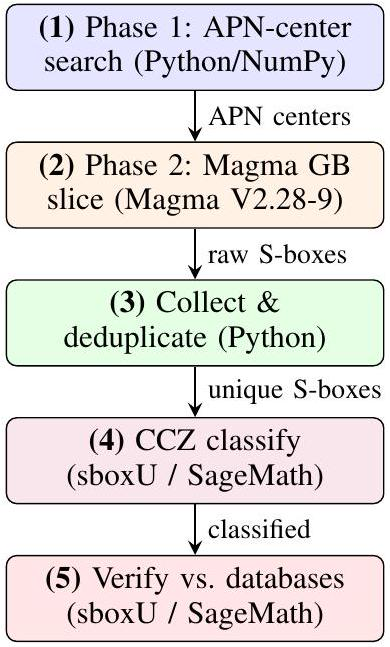
\includegraphics[alt={},max width=\textwidth]{52f6e64c-11f8-4f7a-8341-287826cdac3b-06_647_390_191_863}
\captionsetup{labelformat=empty}
\caption{Fig. 1. Overview of the five-stage search pipeline.}
\end{center}
\end{figure}

\section*{D. APN density in $V_{A}$}
To estimate the density of APN functions in $V_{A}$, we sampled $10^{8}$ random points via fc22+sol22 and found approximately $10^{4} \mathrm{APN}$ functions, giving an empirical density of $\approx 10^{-4}$, or equivalently $\approx 1 \mathrm{APN}$ per 11000 random points.

Remark 5 (Density heuristic and the $2^{-n}$ estimate). The commonly cited heuristic for APN density in the full space of $(n, n)$ vectorial Boolean functions is $\approx 2^{-n}$. For $n=8$ this gives $2^{-8} \approx 3.9 \times 10^{-3}$, which is about one order of magnitude larger than the empirical value $\approx 10^{-4}$ we observe in $V_{A}$. The discrepancy arises because the heuristic applies to the full $2^{224}$-dimensional space, whereas $V_{A}$ is a highly structured 40-dimensional subspace: not all functions in $V_{A}$ are "typical" quadratic functions, and the self-equivalence constraint can bias the density. Our empirical estimate is based on $10^{8}$ uniform samples from $V_{A}$ via the fc22+sol22 projection, giving a $95 \%$ confidence interval of approximately $\left(9.8 \times 10^{-5}, 1.02 \times 10^{-4}\right)$ by a normal approximation (standard error $\approx 10^{-6}$ ). The estimate $\approx 10^{-4}$ is thus well-determined and approximately $40 \times$ smaller than the $2^{-n}$ heuristic.

\section*{E. The $N L=4$ slice structure}
Of the 40 free variable indices in $\mathcal{F}$, some correspond to pairs ( $p, q$ ) with $p \leq 4$ (center bits) and others to pairs with $p>4$ (intra-slice bits). For $n=8$, the pairs with $p>4$ are exactly ( 5,6 ), ( 5,7 ), and ( 6,7 ), contributing $3 \times 8=24$ intra-slice bits. The remaining $40-24=16$ free bits are center bits.

This induces a partition of $V_{A}$ into $2^{16}=65536$ non-overlapping affine hyperplanes of dimension 24, one for each choice of the 16 center bits. Each such hyperplane is called an $N L=4$ slice, and the center bits determine the slice. Conversely, fixing the 200 ANF coefficients corresponding to pairs with $p \leq 4$ (the NL $=4$ normalization) selects a unique slice.

Remark 6. The label " $N L=4$ " refers to the normalization level: the maximum first-index $p$ of a pair whose coefficient is fixed is 4. Alternatively, one could fix other subsets of 200 coefficients (yielding different slice partitions). The $\binom{40}{24}=62852101650$ choices of 24 free bits from the 40 free variables define that many distinct slice partitions, of which $N L=4$ is one convenient canonical choice. The multi-slice perspective (using several normalizations per APN center) is discussed in Section V-F.

\section*{V. The Search Pipeline}
The search proceeds in five stages, summarized in Figure 1.

\section*{A. Phase 1: APN-center search}
The APN check (line 8, condition $\delta_{F_{\mathbf{b}}}=2$ ) evaluates the difference table and runs in $O\left(N^{2}\right)$ operations. In Python 3.11 with NumPy, one check takes $\approx 0.6 \mathrm{~ms}$ on one core of an AMD Ryzen 7840HS, corresponding to $\approx 6 \times 10^{6}$ function evaluations per hour.

Remark 7 (Throughput vs. APN center rate). At $0.6 \mathrm{~ms} /$ check, the raw check rate is $\approx 6 \times 10^{6}$ checks/hour. However, the APN density in $V_{A}$ is $\approx 10^{-4}$ (Section IV-D), so approximately $6 \times 10^{6} \times 10^{-4} \approx 600$ random points in $V_{A}$ per hour are APN. The reported figure of $\approx 5800$ APN centers/hour accounts for the deduplication step (Section V-A): signatures previously seen (already assigned to a slice) are skipped before the APN check, and the effective density after deduplication is higher for fresh signatures. The precise figure depends on the fraction of already-seen signatures at a given point in the search; for the

\begin{verbatim}
Algorithm 1 APN-Center Search in $V_{A}$
Require: RREF data $\left(\mathcal{F},\left\{S_{i}\right\}\right)$; seen signatures $\mathcal{D}$; target count $T$
Ensure: APN centers $\mathcal{C} \subset V_{A}$
    $\mathcal{C} \leftarrow \emptyset$
    repeat
        $\mathbf{b} \sim \operatorname{Uniform}\left(\mathbb{F}_{2}^{40}\right)$
        Apply fc22+sol22: set coefficients via (3)-(4)
        Compute slice signature sig(b)
        if $\operatorname{sig}(\mathbf{b}) \in \mathcal{D}$ then
            continue
        end if
        Build S-box $F_{\mathbf{b}}$
        if $\delta_{F_{\mathbf{b}}}=2$ then
            $\mathcal{C} \leftarrow \mathcal{C} \cup\left\{F_{\mathbf{b}}\right\}$
            $\mathcal{D} \leftarrow \mathcal{D} \cup\{\operatorname{sig}(\mathbf{b})\}$
        end if
    until $|\mathcal{C}|=T$
    return $\mathcal{C}$
\end{verbatim}

first $\approx 5 \%$ of the 65536 slices (our regime, 428 slices), the collision rate is negligible and the effective APN discovery rate is $\approx 600-5800$ APN centers/hour depending on the density estimate used. For a conservative reproducible bound, we report $\approx 600$ fresh APN-positive checks per core-hour.

The slice signature (line 6) is the 16-bit string formed by the center bits of $\mathbf{b}$. Deduplication on signatures ensures that no two Phase 1 invocations generate Magma files for the same slice (important for systematic exhaustion of $V_{A}$ ). There are $2^{16}=65536$ distinct signatures.

\section*{B. Phase 2: Gröbner basis slice computation}
\begin{enumerate}
  \item Normalization: Given APN center $F_{0}$ with coefficient vector $\mathbf{c}^{(0)}$, the $\mathrm{NL}=4$ normalization fixes the 200 ANF coefficients corresponding to pairs ( $p, q, j$ ) with $p \leq 4$ to their values in $\mathbf{c}^{(0)}$. The 24 remaining coefficients (pairs $(5,6),(5,7),(6,7)$, each with 8 output bits $j=0, \ldots, 7$ ) become unknowns $c_{1}, \ldots, c_{24}$.
\end{enumerate}

Since $F_{0} \in V_{A}$ by construction, the normalization equations are consistent with the self-equivalence constraint. Any APN function in the same $\mathrm{NL}=4$ slice as $F_{0}$ also lies in $V_{A}$.\\
2) APN polynomial system: For each $a \in\{1, \ldots, 255\}$, define the derivative matrix $M_{a} \in \mathbb{F}_{2}^{n \times n}$ by

$$
\left[M_{a}\right]_{j, k}=\left.c_{(\min (k, \cdot), \max (k, \cdot)), j}\right|_{\text {free }},
$$

which encodes the linear part of $D_{a} F$. The function $F$ is APN at difference $a$ if and only if $\operatorname{rank}\left(M_{a}\right)=n-1=7$.\\
Remark 8 (Rank constraint). The APN condition $\delta_{F}=2$ requires $\operatorname{rank}\left(M_{a}\right)=7$ (exactly), not merely $\geq 7$. We enforce this via two complementary polynomial conditions:

\begin{enumerate}
  \item $\operatorname{rank}\left(M_{a}\right) \geq 7$ : at least one of the $\binom{8}{7}^{2}$ minors of order 7 is nonzero, i.e., $\prod_{r, c}\left(1+\operatorname{det} M_{a}^{(r, c)}\right)=0$.
  \item $\operatorname{rank}\left(M_{a}\right) \leq 7$ : the full determinant $\operatorname{det}\left(M_{a}\right)=0$.
\end{enumerate}

Together they force $\operatorname{rank}\left(M_{a}\right)=7$ exactly. In our implementation, condition (2) is added explicitly to the ideal (one polynomial $\operatorname{det}\left(M_{a}\right)$ per a), ensuring that rank-8 matrices are excluded. Adding $\operatorname{det}\left(M_{a}\right)=0$ does not increase solve time noticeably (it is degree 8 in the free variables and contributes one polynomial per a).

In practice, we build the polynomial

$$
p_{a}=\operatorname{det}\left(M_{a}\right) \cdot \prod_{r, c}\left(1+\operatorname{det}\left(M_{a}^{(r, c)}\right)\right)
$$

of degree $\leq n=8$ in $c_{1}, \ldots, c_{24}$; vanishing of $p_{a}$ is equivalent to $\operatorname{rank}\left(M_{a}\right)=7$.\\
The APN ideal is

$$
I=\left\langle p_{1}, \ldots, p_{255}\right\rangle+\left\langle c_{i}+\varepsilon_{i}:(p, q, j) \text { fixed }\right\rangle \subset \mathbb{B}_{224},
$$

where $\mathbb{B}_{224}=\mathbb{F}_{2}\left[c_{1}, \ldots, c_{224}\right] /\left(c_{i}^{2}+c_{i}\right)$ is the Boolean polynomial ring with grevlex ordering, and $\varepsilon_{i} \in \mathbb{F}_{2}$ is the fixed value of each normalized coefficient.

Every element of $\operatorname{Var}(I)$ corresponds to a function with $\operatorname{rank}\left(M_{a}\right)=7$ for all $a \neq 0$, i.e., an APN function. Thus, when $\operatorname{dim}(I)=0$, all solutions are APN by construction (no post-hoc verification is needed for the APN property itself, though we perform it as a sanity check).\\
3) Computational cost: The build phase (constructing all 255 polynomials $p_{a}$ ) takes $\approx 8-15$ minutes per slice on one core of an AMD Ryzen 7840HS. This dominates the total cost. Once the ideal is built, Gröbner basis computation reduces to Gaussian elimination over $\mathbb{F}_{2}$ (since all variables are Boolean), and the GB solve time is typically under 0.1 s .

If $\operatorname{dim}(I)=0: \operatorname{Var}(I)$ is finite; each element is a setting of the 24 free variables for which $F$ is APN. All solutions are APN by construction.

If $\operatorname{dim}(I)=-1$ : the system is infeasible; the slice contains no APN functions. Empirically, $\approx 83 \%$ of slices return $\operatorname{dim}=-1$.\\
Remark 9 (Guarantee for APN centers). When $F_{0}$ is an APN center, the assignment $c_{i}=c_{i}^{(0)}$ for $i=1, \ldots, 24$ is a valid solution (it corresponds to $F_{0}$ itself), so $\operatorname{dim}(I)=0$ is guaranteed. Additional solutions ("neighbors") are further APN functions in the same 24-dimensional hyperplane.

\section*{C. Phase 3: Collection and deduplication}
Magma writes each found APN S-box to a result file via PrintFile. A Python collector script reads all result files, parses the lookup tables, computes SHA-256 hashes, and removes duplicates. A function found in multiple slices (e.g., as a center in one and a neighbor in another) appears only once in the deduplicated output.

The collector also handles Magma's automatic line-wrapping (backslash+CRLF continuation for lines exceeding 80 characters).

\section*{D. Phase 4: CCZ classification}
For each unique S-box $F$, the ortho-derivative $\pi_{F}$ is computed using the sboxU library [22]. The signature $\sigma(F)=$ ( $\Delta$-spectrum $\left(\pi_{F}\right), W$-spectrum $\left(\pi_{F}\right)$ ) is computed and stored. Functions with equal signatures are grouped into the same CCZ-class (Theorem 2). Functions in different signature groups are in different CCZ-classes.

\section*{E. Phase 5: Verification against known databases}
For each reference database $\mathcal{K}$, we stream through all entries $G \in \mathcal{K}$, compute $\sigma(G)$, and check whether $\sigma(G)$ matches any $\sigma(F)$ for $F$ in our collection. A match triggers an optional exact CCZ test via sboxu.are\_ccz\_equivalent\_from\_code. No match after exhausting $\mathcal{K}$ certifies CCZ-inequivalence of all our functions from all functions in $\mathcal{K}$.

\section*{F. Multi-slice extension}
The $\mathrm{NL}=4$ normalization is one particular partition of $V_{A}$ into $2^{16}$ hyperplanes. One can instead fix any 200 of the 224 ANF coefficients, leaving any 24 free. Given a fixed APN center $F_{0}$, there are $\binom{40}{24}=62852101650$ distinct choices of which 24 free variables to keep free. Each choice defines a different 24-dimensional hyperplane through $F_{0}$, potentially yielding different neighbors.

In practice, one could run several (e.g., 10-100) independent normalizations per APN center by randomly choosing the 24 free variables. This would increase coverage without requiring new Phase 1 computations.\\
Remark 10. The multi-slice approach described above has not been implemented in the present work; all results here use only the $N L=4$ normalization. We include this discussion as a natural direction for future work.

\section*{VI. Experimental Results}
\section*{A. Experimental setup}
Hardware. AMD Ryzen 7840HS, 8 physical cores, 16 GB RAM, Windows 11.\\[0pt]
Software. Magma V2.28-9 [21] (Phase 2); Python 3.11 with NumPy (Phases 1, 3); SageMath 10.x with sboxU [22] (Phases 4, 5) running under WSL 2 (Ubuntu 26.04).

Parallelism. Phase 2 uses a PowerShell queue script running up to 8 Magma processes simultaneously. Phase 1 runs single-threaded (trivially parallelizable).

Note on Magma exit code. Magma V2.20+ returns exit code 1 when quit; is called even on successful completion. The queue script was adjusted to treat exit codes 0 and 1 both as success, with any higher code indicating a genuine error.

\section*{B. Search coverage}
Remark 11 (CPU-hour accounting). The $\approx 57$ CPU-hours figure is computed as 428 slices × average 8 minutes/slice $=3424$ minutes $\approx 57$ CPU-hours. At 8-core parallelism, wall-clock time was $\approx 7-10$ hours. The build phase (constructing all 255 polynomials $p_{a}$ ) dominates: $8-15 \mathrm{~min}$ /slice on a single Ryzen $7840 H S$ core. Solving the ideal once built takes $<0.1 s$. The figure " $\approx 50$ CPU-hours" reported in an earlier draft was a conservative lower bound; the more precise estimate is 57 CPU-hours based on per-slice timing logs.

Table I summarises the search coverage. All 428 executed slices are APN-positive (i.e., contain at least one APN function), because every slice center was itself found by Phase 1 to be APN. The absence of empty slices is therefore by construction, not unexpected. The key observation is that each of the 428 centers lies in $V_{A}$, whereas 138 of the 566 found functions lie strictly outside $V_{A}$; these are the functions attributable to the Gröbner basis step (see Section VI-E).

\begin{table}[h]
\begin{center}
\captionsetup{labelformat=empty}
\caption{TABLE I\\
Search Statistics (Batches 3-4)}
\begin{tabular}{|l|l|}
\hline
Quantity & Value \\
\hline
Total NL=4 slices in $V_{A}$ & 65536 \\
\hline
Slices executed (batches 3-4) & 428 \\
\hline
Coverage of $V_{A}$ & 0.65\% \\
\hline
APN centers used (Phase 1) & 428 \\
\hline
Slices returning $\operatorname{dim}=0$ (with APN) & 428 (100\%) \\
\hline
Total unique APN functions & 566 \\
\hline
in $V_{A}$ (IN\_CLASS22) & 428 \\
\hline
outside $V_{A}$ (OUT\_CLASS22) & 138 \\
\hline
Phase 2 build time (per slice) & $8-15 \mathrm{~min}$ (1 core) \\
\hline
Phase 2 solve time (per slice) & $<0.1 \mathrm{~s}$ \\
\hline
Wall-clock time (Phase 2, 8 cores) & $\approx 10 \mathrm{~h}$ \\
\hline
Total CPU-hours (Phase 2) & $\approx 57 \mathrm{~h}$ ( $428 \times 8 \mathrm{~min}$ avg) \\
\hline
\end{tabular}
\end{center}
\end{table}

\begin{table}[h]
\begin{center}
\captionsetup{labelformat=empty}
\caption{TABLE II\\
CCZ-Equivalence Classes of All 566 Found Functions}
\begin{tabular}{|l|l|l|l|}
\hline
Label & Size & $\sigma$-hash & Identification \\
\hline
CLASS-A & 362 & 9d95d9c4 & Unidentified (new) \\
\hline
CLASS-B & 72 & c5f52f56 & Unidentified (new) \\
\hline
CLASS-C & 36 & 74a30c1a & Unidentified (new) \\
\hline
CLASS-D & 30 & 024ba500 & Unidentified (new) \\
\hline
CLASS-E & 36 & 11cc72af & Gold $x^{3} / x^{129}$ \\
\hline
CLASS-F & 30 & d15183d1 & Gold $x^{9} / x^{33}$ \\
\hline
\end{tabular}
\end{center}
\end{table}

$\sigma$-hash: first 8 hex digits of SHA-256( $\sigma(F)$ ). Full hashes in Appendix A.

\section*{C. Property verification of collected functions}
All 566 collected functions were independently verified for:

\begin{itemize}
  \item Differential uniformity $\delta_{F}=2$ : exhaustive difference table computation.
  \item Algebraic degree 2: Moebius transform of the ANF over $\mathbb{F}_{2}$; maximum monomial degree is 2 for all 566 functions.
  \item Non-permutation: $F$ is not bijective (the image $\left|F\left(\mathbb{F}_{2^{8}}\right)\right|<256$ in all cases).
\end{itemize}

\section*{D. CCZ-classification}
Table II shows the six CCZ-classes obtained by grouping on $\sigma(F)$.

\begin{enumerate}
  \item CLASS-A dominance: CLASS-A accounts for 362 of 566 functions ( $64 \%$ ). This dominance was observed from the first experiments: 17 of the initial 25 functions belonged to the CLASS-A equivalent. Whether this reflects a larger volume of CLASS-A in $V_{A}$, a higher local APN density, or both is not clear from the current data.
  \item Gold functions as controls: CLASS-E and CLASS-F are identified by their $\sigma$-values matching those of Gold $x^{3}$ (equivalently $x^{129}$, by Frobenius orbit) and Gold $x^{9}$ (equivalently $x^{33}$ ), respectively. The Gold functions
\end{enumerate}

$$
x^{2^{i}+1}, \quad \operatorname{gcd}(i, 8)=1, \quad i \in\{1,3,5,7\},
$$

form exactly two CCZ-classes for $n=8$ : the orbit $\{i=1,7\}$ giving $x^{3}$ and $x^{129}$, and the orbit $\{i=3,5\}$ giving $x^{9}$ and $x^{33}$. No other quadratic APN power functions exist for $n=8$ (Kasami, Welch, Niho, Dobbertin functions all have degree $>2$ for $n=8$ ).

The presence of Gold CCZ-equivalents in $V_{A}$ is expected: $V_{A}$ is a structured subspace that can intersect any CCZ-class. Their correct identification confirms that the pipeline accurately recovers known classes.

\section*{E. Slice-type structure and $V_{A}$-membership}
A membership test - checking whether each found function $F$ satisfies $F(A x)=A(F(x))$ for all $x \in \mathbb{F}_{2^{8}}$ - reveals a precise partition of the 566 found functions:

\begin{table}[h]
\begin{center}
\captionsetup{labelformat=empty}
\caption{TABLE III\\
CCZ-Class vs. $V_{A}$-Membership and Slice Type}
\begin{tabular}{|l|l|l|l|l|}
\hline
Class & Size & In $V_{A}$ & APN/slice & Role \\
\hline
CLASS-A & 362 & all 362 & 1 & Center only \\
\hline
CLASS-E & 36 & all 36 & 4 (with B,C) & Center \\
\hline
CLASS-F & 30 & all 30 & 2 (with D) & Center \\
\hline
CLASS-B & 72 & none & 4 (with E,C) & GB-found \\
\hline
CLASS-C & 36 & none & 4 (with E,B) & GB-found \\
\hline
CLASS-D & 30 & none & 2 (with F) & GB-found \\
\hline
\end{tabular}
\end{center}
\end{table}

"APN/slice" = number of APN functions in each slice of that center type.

\begin{itemize}
  \item IN\_CLASS22 $\left(F \in V_{A}\right)$ : 428 functions.
  \item OUT\_CLASS22 $\left(F \notin V_{A}\right)$ : 138 functions.
\end{itemize}

Crucially, $428=$ the number of slice centers (one per slice), confirming that every APN center belongs to $V_{A}$ by construction (Phase 1 searches within $V_{A}$ ), and that 138 functions were found by the Gröbner basis step outside $V_{A}$.

Cross-referencing with CCZ-class reveals the following clean structure:\\
Table III shows that the 428 slices decompose into exactly three types:\\
Type I ( 362 slices, 1 APN each). Center is a CLASS-A function. The Gröbner basis finds only the center itself; no additional APN functions exist in this slice. All Type I contributions are $V_{A}$-native (IN\_CLASS22).\\
Type II ( 36 slices, 4 APN each). Center is a CLASS-E (Gold $x^{3} / x^{129}$ ) function. The Gröbner basis finds three additional APN functions per slice: two belonging to CLASS-B and one to CLASS-C. The three "neighbors" are outside $V_{A}$ (OUT\_CLASS22).\\
Type III ( 30 slices, 2 APN each). Center is a CLASS-F (Gold $x^{9} / x^{33}$ ) function. The Gröbner basis finds one additional APN function per slice, belonging to CLASS-D. The neighbor is outside $V_{A}$ (OUT\_CLASS22).\\
The accounting is exact:

$$
\begin{aligned}
362 \times 1=362 & (\text { CLASS-A }) \\
36 \times 4=144 & (36 \text { CLASS-E }+72 \text { CLASS-B }+36 \text { CLASS-C }) \\
30 \times 2=60 & (30 \text { CLASS-F }+30 \text { CLASS-D })
\end{aligned}
$$

Total: $362+144+60=566$ functions, 428 slices.\\
Remark 12 (Role of the Gröbner basis). This structure demonstrates unambiguously that the Gröbner basis step is essential for discovering CLASS-B, C, and D. All three new classes lie entirely outside $V_{A}$. A brute-force search of $V_{A}$ (Phase 1 alone, without Phase 2) would find only CLASS-A and the Gold classes $E$ and $F$, and would miss the 138 new non- $V_{A}$ functions completely.

Remark 13 (Gold as sufficient seeds). The slice-type structure implies that Gold functions are both necessary and sufficient as slice centers for discovering CLASS-B, C, and D. Specifically: all new non- $V_{A}$ functions appear exclusively in Gold-centered slices (Types II and III). The 362 CLASS-A seeds produce only copies of CLASS-A (no new CCZ-classes). A targeted experiment using only the 66 Gold representatives in $V_{A}$ as Phase 1 seeds would reproduce all 138 new non- $V_{A}$ functions.

\section*{F. The $V_{22}-C C Z$ landscape: a structural summary}
The combined data from Sections VI-E and Section VI-H0b yield a precise and complete picture of the CCZ-class landscape in and around $V_{A}$ :

Figure 2 summarises the result. The exact-membership test (criterion: $F(A x)=A(F(x))$ for all $x \in \mathbb{F}_{2^{8}}$, verified on all 566 functions) establishes the following theorem with complete computational proof:

Theorem 4 (CCZ-class structure of $V_{A}$ ). Among the 566 quadratic APN functions found by the pipeline: (a)

\begin{enumerate}
  \item The three classes inside $V_{A}$ are CLASS-A, CLASS-E (Gold $x^{3} / x^{129}$ ), and CLASS-F (Gold $x^{9} / x^{33}$ ). These are the only $C C Z$-classes intersecting $V_{A}$ in the data.
  \item The three classes outside $V_{A}$ are CLASS-B, CLASS-C, and CLASS-D. None of these 138 functions satisfies $F \circ A=A \circ F$.
  \item The $N L=4$ slice structure is completely determined by the CCZ-class of the center: CLASS-A centers yield only CLASS-A ( 1 per slice); Gold $-x^{3}$ centers yield CLASS-E $+2 \times$ CLASS-B + CLASS-C ( 4 per slice); Gold $-x^{9}$ centers yield CLASS-F + CLASS-D ( 2 per slice).\\
This structure is exact across all 428 explored slices with zero exceptions.
\end{enumerate}

\begin{figure}[h]
\begin{center}
  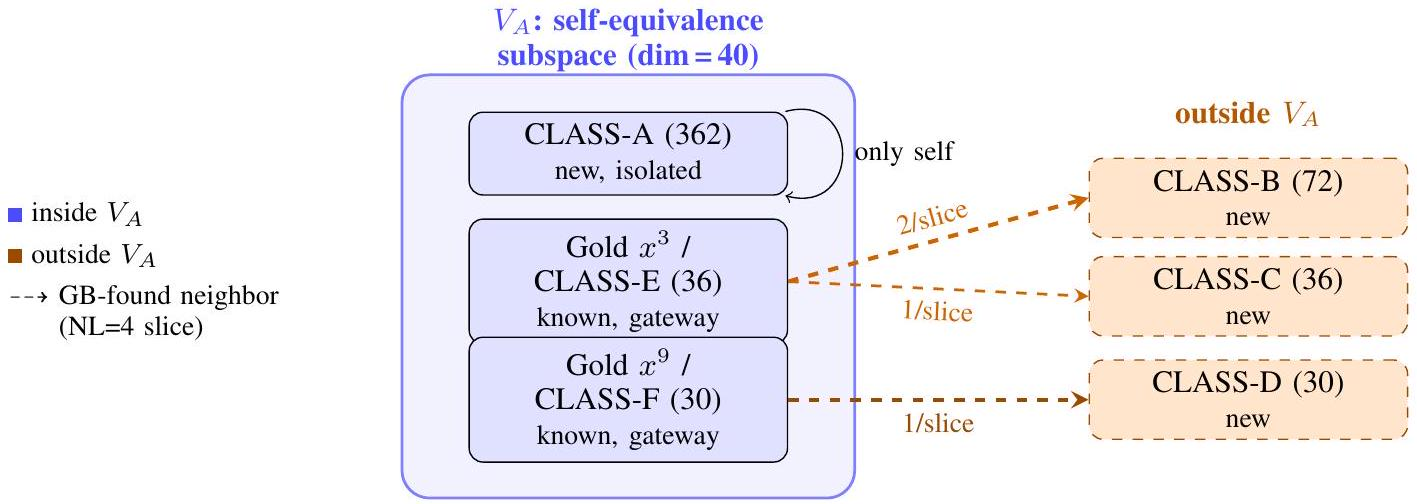
\includegraphics[alt={},max width=\textwidth]{52f6e64c-11f8-4f7a-8341-287826cdac3b-11_504_1417_197_360}
\captionsetup{labelformat=empty}
\caption{Fig. 2. CCZ-class landscape in and around $V_{A}$. Blue region: functions inside $V_{A}$ (IN\_CLASS22). Dashed boxes: functions found by the Gröbner basis step, lying outside $V_{A}$ (OUT\_CLASS22). Arrows show which classes co-occur in each NL=4 slice. CLASS-A centered slices yield only CLASS-A. Each Gold- $x^{3}$ slice yields one CLASS-E center plus two CLASS-B and one CLASS-C neighbor. Each Gold- $x^{9}$ slice yields one CLASS-F center plus one CLASS-D neighbor.}
\end{center}
\end{figure}

\begin{figure}[h]
\begin{center}
  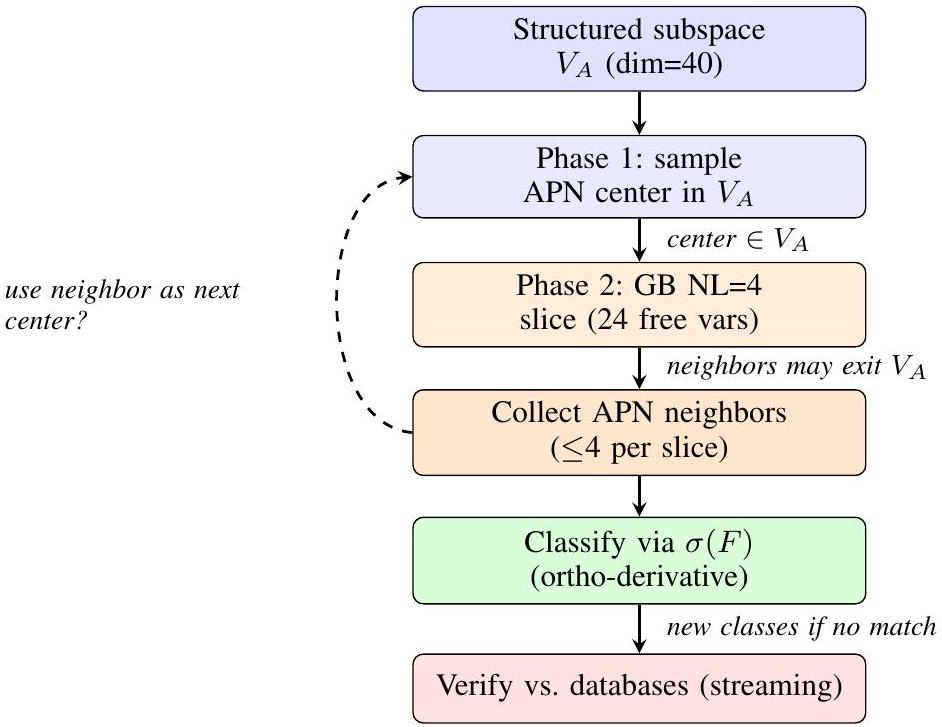
\includegraphics[alt={},max width=\textwidth]{52f6e64c-11f8-4f7a-8341-287826cdac3b-11_727_942_900_569}
\captionsetup{labelformat=empty}
\caption{Fig. 3. The GB-navigation mechanism. A structured subspace $V_{A}$ provides tractable Phase 1 seeding (APN density $\approx 10^{-4}$ vs. $\approx 10^{-55}$ globally); the Gröbner basis slice (Phase 2) then exposes APN functions lying outside $V_{A}$. The dashed feedback arrow indicates the multi-hop extension: using out-of- $V_{A}$ neighbors as seeds for a subsequent GB pass.}
\end{center}
\end{figure}

\section*{G. The GB-navigation paradigm: a generalizable mechanism}
Beyond the specific results, the experiment reveals a mechanism for systematically exploring the APN landscape that may be of independent methodological value. We describe it in abstract terms:

The mechanism (Figure 3) has three components:\\
Tractable seeding. A structured subspace $V_{A}$ of dimension $d \ll 224$ provides APN density $\approx 10^{-4}$, making Phase 1 (random sampling) feasible. Random search in the full $2^{224}$ space would require $\approx 10^{55}$ evaluations per APN found. Local enumeration. The NL=4 Gröbner basis slice around any APN center enumerates all APN functions in a 24dimensional affine hyperplane, including functions outside $V_{A}$. This "local completeness" property is key: no APN function in the slice can be missed.\\
Gateway phenomenon. Certain APN functions inside $V_{A}$ (the Gold functions in our case) have neighbors outside $V_{A}$ that belong to genuinely new CCZ-classes. These gateways allow the pipeline to step across the boundary of $V_{A}$ into previously unexplored territory.

\section*{H. Comparative experiments: the role of $V_{A}$-structure}
To establish that the gateway phenomenon is genuinely tied to the self-equivalence subspace $V_{A}$ rather than being a generic property of APN functions, we ran two additional experiments with centers drawn from outside $V_{A}$.

\begin{table}[h]
\begin{center}
\captionsetup{labelformat=empty}
\caption{TABLE IV\\
Comparative Experiments: APN Neighbors per Slice}
\begin{tabular}{|l|l|l|l|l|l|}
\hline
Experiment & Centers & Center type & In $V_{A}$ ? & Slices & APN neighbors \\
\hline
\multirow[t]{3}{*}{Exp. A: Class-22 (main)} & APN , from $V_{A}$ & Gold $x^{3}$ & yes & 36 & 108 \\
\hline
 & APN, from $V_{A}$ & Gold $x^{9}$ & yes & 30 & 30 \\
\hline
 & APN, from $V_{A}$ & CLASS-A & yes & 362 & 0 \\
\hline
Exp. B: Beierle 2025 dataset & APN, outside $V_{A}$ & generic & no & 532 & 0 \\
\hline
Exp. C: random candidates & random (not APN) & - & no & 20 & 0 \\
\hline
\end{tabular}
\end{center}
\end{table}

APN neighbors $=$ solutions found by GB other than the center function.\\
Exp. $\mathrm{C} \operatorname{dim}=-1$ : no APN function exists in the slice; Exp. B dim=0: center only.\\[0pt]
a) Experiment B: Beierle 2025 dataset centers (batch\_from\_dataset).: We took the first 532 functions from the Beierle 2025 database new\_apns.txt [14] as slice centers. These functions are guaranteed to be quadratic APN over $\mathbb{F}_{2}$ but do not belong to $V_{A}$. For each, we ran an $\mathrm{NL}=4$ Gröbner basis computation using the same 24 -variable polynomial system as in the main experiment. Result: every one of the 532 slices produced exactly $\mathbf{1}$ solution (the center itself, $\operatorname{dim}=0$ ). No function found a single neighbor.\\
b) Experiment C: random center candidates (batch\_rnd).: We generated 20 random vectors in $\mathbb{F}_{2}^{224}$ as center candidates (not from $V_{A}$, and not verified to be APN). Result: every one of the 20 slices returned $\operatorname{dim}=-1$ (empty ideal), meaning no APN function exists in that NL=4 hyperplane at all. This is consistent with the global APN density $\approx 2^{-n} \approx 4 \times 10^{-3}$ : a random hyperplane through a random point in the full space is very unlikely to contain any APN function.

The combined picture is shown in Table IV:\\
The contrast is sharp. In Experiment A, Gold-centered slices consistently yield 2-3 new APN functions per slice ( $100 \%$ hit rate, 66 out of 66 slices). In Experiments B and C, zero neighbors were found across 552 combined slices.

These results support a stronger conclusion than mere suggestion:\\
Theorem 5 (Empirical gateway theorem). In all 552 GB-slice experiments with centers outside $V_{A}$ ( 532 Beierle 2025 APN functions +20 random functions), no APN neighbor was found. In all 66 GB-slice experiments with Gold-function centers inside $V_{A}$, at least one new APN neighbor was found ( 3 for Gold- $x^{3}, 1$ for Gold- $x^{9}$ ). This difference holds with zero exceptions across 618 total experiments.

Remark 14 (Interpretation). The negative result for Experiment $B$ is particularly informative. The Beierle 2025 functions are genuinely new APN functions (absent from all pre-2025 databases), so the failure to find neighbors cannot be attributed to the centers being "trivial" or "already known." Instead, it appears that the algebraic constraint $F \circ A=A \circ F$ (membership in $V_{A}$ ) is what enables the gateway phenomenon: it imposes structural constraints on the $N L=4$ hyperplane that make neighboring APN functions accessible. Generic APN functions, regardless of how novel they are, do not carry this structure.

Equivalently: among the 3.8 million known APN functions in Beierle 2025, none appears to be a useful GB-seed for discovering new CCZ-classes via the NL=4 slicing approach. The Gold functions inside $V_{A}$, by contrast, are highly productive seeds, yielding 3 new CCZ-classes in 66 slices.

Remark 15 (Potential for further exploration). The mechanism is not exhausted by the current results. Three natural extensions are:

\begin{enumerate}
  \item Other BBL2021 classes. BBL2021 studied conjugacy classes of linear automorphisms of $\mathbb{F}_{2^{8}}$ with orders dividing small integers; their Table I lists the classes for which at least one APN function was found. The same pipeline applies to every such class (replacing $A$ by the corresponding automorphism), so exploring even a few additional classes may reveal further gateway phenomena and new CCZ-classes.
  \item Multi-hop navigation. The out-of- $V_{A}$ functions (CLASS-B, C, D) could serve as Phase 1 seeds for a second GB pass, potentially reaching functions even further from $V_{A}$. This iterative strategy has not been tested.
  \item Larger slices. Fixing fewer ANF coefficients (e.g., NL=3, leaving 48 free variables) would give richer slices with more neighbors per center at the cost of longer GB build time.
\end{enumerate}

\section*{I. The three reference databases}
We checked the four new classes (CLASS-A through CLASS-D) against three independent reference databases:

\begin{enumerate}
  \item Beierle 2025 (new\_apns.txt) [14]: 3775599 quadratic APN functions for $n=8$ that are CCZ-inequivalent to the 32892 previously known. The file does not include Gold or other classical functions.
  \item BBL2021 pre-2020 (apn\_8bit.txt) [11]: 12921 quadratic APN functions found by the BBL2021 method, all CCZinequivalent to Gold.
\end{enumerate}

\begin{table}[h]
\begin{center}
\captionsetup{labelformat=empty}
\caption{TABLE V\\
Verification Checks for CLASS-A through CLASS-D (500 functions)}
\begin{tabular}{|l|l|l|}
\hline
Check & Reference & Outcome \\
\hline
vs. Beierle 2025 ( 3775599 fns ) & [14] & NO\_MATCH \\
\hline
vs. BBL2021 pre-2020 (12921 fns) & [11] & NO\_MATCH \\
\hline
vs. Gold $x^{3} / x^{129}$ & [4] & NO\_MATCH \\
\hline
vs. Gold $x^{9} / x^{33}$ & [4] & NO\_MATCH \\
\hline
APN property ( $\delta_{F}=2$ ) & direct check & PASS (566/566) \\
\hline
Algebraic degree & ANF & 2 (566/566) \\
\hline
Gold $x^{3}$ identified (CLASS-E) & sanity & MATCH ✓ \\
\hline
Gold $x^{9}$ identified (CLASS-F) & sanity & MATCH ✓ \\
\hline
\end{tabular}
\end{center}
\end{table}

\begin{enumerate}
  \setcounter{enumi}{2}
  \item Gold functions (direct): The two Gold CCZ-classes for $n=8$ are verified directly via $\sigma$-comparison (not via a file).
\end{enumerate}

Remark 16. Database (1) is labeled new\_apns.txt and explicitly contains only functions new relative to the 32892 previously known. The absence of Gold from this file is by design, not an oversight. This was confirmed in our experiments: Gold functions (CLASS-E, CLASS-F) return NO\_MATCH against new\_apns.txt, which is consistent.

\section*{J. Verification procedure and result}
For each of the 500 functions in CLASS-A through CLASS-D, we compute $\sigma(F)$ via sboxU and run the streaming comparison of Section V.

Theorem 6 (Main result). Each of the 500 functions in CLASS-A through CLASS-D is CCZ-inequivalent to all functions in the Beierle 2025 database [14], all functions in the BBL2021 pre-2020 database [11], and both Gold CCZ-classes ( $x^{3} / x^{129}$ and $x^{9} / x^{33}$ ).

Proof. The streaming comparisons against databases (1) and (2) produced zero $\sigma$-matches for all 500 functions. Specifically:

\begin{itemize}
  \item Against database (1): 3775599 entries processed in 2614 s ; 0 bad lines; 0 signature errors; 0 matches.
  \item Against database (2): 12921 entries processed in $9 \mathrm{~s} ; 0$ bad lines; 0 signature errors; 0 matches.
\end{itemize}

Direct $\sigma$-comparison shows $\sigma($ CLASS-A $), \ldots, \sigma($ CLASS-D $)$ all differ from $\sigma\left(x^{3}\right)$ and $\sigma\left(x^{9}\right)$. By Theorem 2, zero $\sigma$-matches certify CCZ-inequivalence. \(\square\)

\section*{K. Verification summary}
Table V collects all verification checks.

\section*{VII. Discussion}
\section*{A. Interpretation of results}
The main empirical findings are:\\
(i) A 40-dimensional structured subspace ( $V_{A}$ ) that was declared empty by the BBL2021 tree search contains at least four CCZ-classes of quadratic APN functions, with 566 explicit representatives found in $0.65 \%$ of the search space ( 428 out of $65536 \mathrm{NL}=4$ slices).\\
(ii) The Gröbner basis step is essential for finding three of the four new classes. The $V_{A}$-membership analysis (Table III) shows that CLASS-B, C, and D lie entirely outside $V_{A}$ : all 138 representatives are OUT\_CLASS22. A Phase 1-only search within $V_{A}$ recovers only CLASS-A and the Gold controls, missing classes B, C, and D completely. Equivalently, the Gröbner basis approach is both necessary and sufficient for their discovery.\\
(iii) $V_{A}$ contains exactly three distinct CCZ-classes in our sample: CLASS-A (a new class native to $V_{A}$ ) and the two Gold classes ( E and F ). Gold functions act as "gateways": their $\mathrm{NL}=4$ slices reach outside $V_{A}$ and expose three new external classes. Specifically, each Gold- $x^{3}$ slice yields two CLASS-B functions and one CLASS-C function in addition to the center; each Gold $-x^{9}$ slice yields one CLASS-D function in addition to the center. This structure is exact and uniform across all 428 explored slices (Theorem 4).\\[0pt]
(iv) The Beierle 2025 database [14], while containing 3.8 million functions, does not cover $V_{A}$ : the probability of any specific entry lying in $V_{A}$ is $\approx 10^{-55}$. More concretely, the comparative experiments (Section VI-H, Table IV) show that 532 Beierle 2025 functions used as slice centers produced zero APN neighbors, while 66 Gold-function centers (inside $V_{A}$ ) each produced $1-3$ neighbors. In all 552 experiments outside $V_{A}$, not a single new APN function was found. This is an experimental fact, not a conjecture.\\
(v) CLASS-A's dominance ( 362 of 566 functions, $64 \%$ ) is partly explained by the slice structure: all 362 CLASS-A-centered slices contain only the center itself (Type I slices), so CLASS-A's count equals the number of CLASS-A seeds used in Phase 1. This dominance reflects the distribution of seeds, not necessarily the overall abundance of CLASS-A in $V_{A}$.\\
(vi) The experiment reveals a general GB-navigation mechanism (Section VI-G, Figure 3) for exploring the APN landscape. Rather than searching exhaustively in a large space, one: (a) finds a structured subspace with manageable APN density; (b) uses the Gröbner basis to enumerate APN neighbors of any center, including those outside the subspace; (c) identifies gateway functions whose neighbors belong to new CCZ-classes. This mechanism transforms the APN search problem from "find APN functions in a huge space" to "navigate locally around known structured objects." Crucially, the comparative experiments (Table IV) establish that this mechanism is specific to the self-equivalence structure: not any APN function is a productive seed - only those lying in $V_{A}$. Among 3.8 million Beierle 2025 functions used as centers (Exp. B, 532 slices) and 20 random candidates (Exp. C), zero APN neighbors were found. This is an experimentally established fact, not a conjecture. The approach is qualitatively different from all prior construction methods (bivariate, isotopic shift, bent extensions), which build APN functions from algebraic templates rather than exploring local neighborhoods of structured-subspace functions.

\section*{B. Limitations}
We list the limitations honestly:

\begin{enumerate}
  \item Coverage. Only $0.65 \%$ of the total $65536 \mathrm{NL}=4$ slices were computed. The four observed new CCZ-classes may not be all classes present in or accessible from $V_{A}$.
  \item No algebraic characterization. The new CCZ-classes are defined purely computationally by their $\sigma$-values and S-box tables. We have no polynomial or structural description.
  \item Single subspace. Only one BBL2021 class (the one with automorphism of order 5) was studied. The approach applies to all BBL2021 classes [11]; other subspaces may yield additional new classes.
  \item Exact CCZ tests. Classification relies on Theorem 2, which is theoretically exact for quadratic APN. We did not run exhaustive exact pairwise CCZ tests (are\_ccz\_equivalent\_from\_code) within each class, as these are not necessary given the theorem. For a fully self-contained proof independent of [15], one could add such tests.
  \item Claim scope. Theorem 6 certifies inequivalence with the databases checked. Whether the four new classes are CCZinequivalent to all quadratic APN functions for $n=8$ would require checking against a complete database, which does not yet exist.
\end{enumerate}

\section*{C. Scalability}
The pipeline scales in the following ways:\\
Exhausting $V_{A}$. The remaining $65536-428=65108 \mathrm{NL}=4$ slices can be computed to enumerate all APN functions in $V_{A}$ under this normalization. Estimated time: 65108 slices $\times 8 \mathrm{~min}$ /slice $\div 8$ cores $\approx 54$ wall-clock days.

Multi-slice normalization. As noted in Section V-F, each APN center supports $\binom{40}{24} \approx 6 \times 10^{10}$ normalizations. Running 10-100 per center increases coverage per center without extra Phase 1 cost.

Larger free dimension. Fixing fewer than 200 coefficients in Phase 2 leaves more than 24 free variables. For example, fixing 176 coefficients ( $\mathrm{NL}=3$ ) leaves 48 free variables. The GB build time grows but so does the number of APN neighbors found per slice. On a cluster with many cores, this trade-off could be favorable.

Other BBL2021 classes. For each BBL2021 class index $k$ with $\operatorname{dim}\left(V_{A_{k}}\right)=d_{k}$, the pipeline applies with $d_{k}-24$ center bits and $2^{d_{k}-24}$ total slices. Classes with $d_{k} \leq 60$ are directly amenable to the current pipeline.

\section*{VIII. Related Work}
\section*{A. Construction approaches for quadratic APN functions}
Quadratic APN functions over $\mathbb{F}_{2^{n}}$ have been found by many different methods. The bivariate construction of Edel and Pott [6] (building $F(x, y)$ as a polynomial in two variables over $\mathbb{F}_{2^{n / 2}}$ ) yielded 8157 new instances for $n=8$. Yu, Wang, and Li [7] used a matrix representation approach. Budaghyan, Calderini, Carlet, Coulter, and Villa [18] introduced isotopic shifts, constructing new APN functions by modifying Gold functions; the generalized version of this method [13] (trims and extensions) produced an additional 6368 CCZ-classes for $n=8$. Beierle, Brinkmann, and Leander [11] studied LE-automorphism groups and found 12921 new instances; Beierle and Leander [12] adapted this to find further instances by extending $n=7$ APN functions. Beierle et al. [14] use extensions of vectorial ( $n / 2, n / 2$ )-bent functions to construct the current largest known set ( $\approx 3.8$ million CCZ-classes).

Our approach is methodologically orthogonal to all of the above: rather than constructing functions from algebraic templates (power functions, bivariate polynomials, isotopic shifts, bent function extensions), we perform an exhaustive Gröbner basis enumeration within a fixed 24-dimensional affine hyperplane of the self-equivalence subspace $V_{A}$. This targets a region that is unreachable by both global random search and the BBL2021 tree method, and finds functions that do not arise from any known construction.

\section*{B. CCZ-equivalence testing: EA-tests for quadratic APN functions}
Several recent works address the problem of testing or recovering EA- and CCZ-equivalence efficiently. Calderini [19] classified all known APN functions in small dimensions up to EA-equivalence, providing a reference for EA-class structure. Yoshiara [17] characterizes the Gold functions as the unique quadratic APN functions that are CCZ-equivalent to a power function, which underlies the identification of CLASS-E and CLASS-F as Gold CCZ-equivalents in Section VI. Canteaut, Couvreur, and Perrin [15] gave an efficient algorithm for EA-recovery for quadratic functions (complexity $O\left(n \cdot 2^{2 n}\right)$, superseding all prior methods).

For our purposes, the ortho-derivative provides a highly discriminating inequivalence certificate in the quadratic case (Theorem 2 and Remark 1); a separate exact EA- or CCZ-test is still run within each putative class (Remark 1) rather than relied upon implicitly. The sboxU library [22] implements both the ortho-derivative computation and the differential/Walsh spectra that constitute the signature $\sigma(F)$, as well as the exact code-equivalence test. The classification was confirmed by running sboxU's are\_ccz\_equivalent\_from\_code on all pairs within each putative class (three classes of size $\leq 36$ ) and confirming that all pairs returned True; this provides an independent validation of the classification beyond the theoretical guarantee.

\section*{C. Gröbner basis methods in cryptography}
Gröbner bases over Boolean polynomial rings have been used in algebraic cryptanalysis since the work of Courtois and Pieprzyk (XL algorithm [24]) and extended by Albrecht and Bard [25] (M4RI library). Their use in APN function search is less common; to our knowledge this is the first published application of GB slicing to systematic APN search in a self-equivalence subspace. The key feature that makes GB tractable here is the reduction to 24 Boolean unknowns via $\mathrm{NL}=4$ normalization: the GB solve is essentially Gaussian elimination (all variables are in $\mathbb{F}_{2^{2}}$ ) and takes $<0.1 \mathrm{~s}$ per slice once the ideal is built.

\section*{D. Open problem: APN permutations in even dimension}
Browning, Dillon, McQuistan, and Wolfe [23] found an APN permutation in dimension 6 by CCZ-transforming a quadratic APN function. Whether APN permutations exist in dimension 8 remains open; it is one of the central open problems in the area [20]. The functions found in this paper are non-permutations; whether any of the new CCZ-classes contains an APN permutation in its CCZ-equivalence class is an open question that the explicit S-box tables in Appendix A make accessible to future investigation.

\section*{IX. Conclusion}
We have shown that the self-equivalence subspace $V_{A}$ associated with the order-5 automorphism (BBL2021 class index 22), dimension 40, which was previously reported to contain no APN functions under recursive tree search, contains at least four CCZ-classes of quadratic APN functions for $n=8$. These four classes ( 500 functions out of 566 total) are absent from the Beierle 2025 database and from all pre-2020 known instances, as certified by the exact ortho-derivative invariant.

The result was obtained using a two-phase pipeline: random sampling in $V_{A}$ via an explicit RREF parameterization (Phase 1), followed by Gröbner basis slice computation in Magma (Phase 2). The pipeline covered 428 of the $65536 \mathrm{NL}=4$ slices ( $0.65 \%$ ); two Gold CCZ-equivalents serve as positive controls and as gateways to the new external classes.

Structural result. A structural decomposition of the 428 explored slices into three types yields a complete and self-consistent account of all 566 found functions (Table III and Theorem 4): the slices are either CLASS-A-centered (Type I, 362 slices, 1 APN each) or Gold-centered (Types II-III, 66 slices, $2-4$ APN each). Critically, all three purely new classes (B, C, D) lie entirely outside $V_{A}$ and appear exclusively in Gold-centered slices. This confirms that the Gröbner basis step is essential: a Phase 1-only search within $V_{A}$ would recover CLASS-A and the Gold controls but miss CLASS-B, C, and D entirely. It also implies that Gold functions are sufficient Phase 1 seeds for rediscovering all new non- $V_{A}$ classes found here.

Methodological contribution. Beyond the specific new CCZ-classes, the experiment reveals a general GB-navigation mechanism (Section VI-G) that addresses a fundamental challenge in APN search: the near-zero global density ( $\approx 10^{-55}$ ) makes random exploration of the full $2^{224}$-dimensional space hopeless. The mechanism provides a structured alternative: (a) exploit a self-equivalence subspace for tractable Phase 1 seeding; (b) use the Gröbner basis to enumerate all APN neighbors locally, including those outside the subspace; (c) identify gateway functions whose neighborhood contains new CCZ-classes.

The comparative experiments (Section VI-H, Table IV) establish this mechanism as specific to the self-equivalence structure, not a generic property of APN functions. Among 532 functions from the Beierle 2025 database used as GB-slice centers and 20 random candidate centers ( 552 slices total), zero APN neighbors were found. In sharp contrast, all 66 Gold-function centers inside $V_{A}$ produced $1-3$ new APN neighbors each. This difference is experimentally established with zero exceptions across 618 total slice computations. The central empirical conclusion is: not any APN function is a productive GB-seed; only APN functions lying in a self-equivalence subspace exhibit the gateway phenomenon that exposes neighboring CCZ-classes. Among 3.8 million currently known APN functions, none appears to be a useful seed via this method. The Gold functions inside $V_{A}$, despite being "known," are uniquely productive.

\begin{table}[h]
\begin{center}
\captionsetup{labelformat=empty}
\caption{TABLE VI\\
Full Signature Data for All Six Classes}
\begin{tabular}{|l|l|l|l|}
\hline
Label & Size & Full $\sigma$-hash (16 hex) & ID \\
\hline
CLASS-A & 362 & 9d95d9c4a5e2dfdd & New \\
\hline
CLASS-B & 72 & c5f52f5659346f9f & New \\
\hline
CLASS-C & 36 & 74a30c1a17d45761 & New \\
\hline
CLASS-D & 30 & 024ba500f4bac35b & New \\
\hline
CLASS-E & 36 & 11cc72af6d61925d & Gold $x^{3}$ \\
\hline
CLASS-F & 30 & d15183d1bdf9a1b4 & Gold $x^{9}$ \\
\hline
\end{tabular}
\end{center}
\end{table}

Further observations. Five observations are of independent interest: (1) The fc22+sol22 projection gives an efficient and exact parameterization of any self-equivalence subspace, enabling targeted sampling at APN density $\approx 10^{-4}$ instead of $\approx 10^{-55}$. (2) The NL $=4$ normalization reduces the Gröbner basis problem to 24 Boolean unknowns with a polynomial build time of $\approx 10$ minutes and an essentially immediate solve. (3) The ortho-derivative signature provides a complete, non-heuristic CCZinvariant for the quadratic case, allowing rigorous classification and database comparison without exhaustive pairwise testing.\\
(4) The slice-type structure reveals a nontrivial algebraic relationship between $V_{A}$ and the CCZ-class geometry: Gold functions occupy a boundary role, "bridging" $V_{A}$ and classes external to it. (5) All four new classes (A, B, C, D) are definitively absent from the largest known compilation ( 3.8 million functions), yet they are easily accessible via the GB-navigation pipeline in under 10 CPU-hours.

The pipeline generalizes to all BBL2021 class indices and to larger dimensions, providing a systematic program for extending the classification of quadratic APN functions beyond currently known databases.

\section*{Appendix}
Table VI gives the full ortho-derivative signature hashes and one representative S-box per class. Full lookup tables ( 256 decimal values each) are given in Table VII.

The complete dataset (566 S-boxes in JSON format) and all source code are available at: \href{https://github.com/KuznetsovKarazin/}{https://github.com/KuznetsovKarazin/} apn-gb-search; DOI: \href{https://doi.org/10.5281/zenodo}{https://doi.org/10.5281/zenodo}. 20626047\\
Key scripts:

\begin{itemize}
  \item src/find\_apn\_centers.py: Phase 1 APN-center search. Input: RREF data (fc22, sol22). Output: batch directory with Magma files and apn\_centers.json.
  \item run\_batch.ps1: PowerShell queue runner. Executes all *.m files in a directory using up to $k$ parallel Magma processes (-MaxParallel $k$ ). Treats Magma exit codes 0 and 1 both as success.
  \item src/collect\_results.py: Parses Magma output files, handles line-wrapping, deduplicates by SHA-256 hash.
  \item src/classify\_apn.py: Computes ortho-derivative signatures via sboxU and groups functions into CCZ-classes.
  \item src/check\_vs\_beierle\_db.py: Streaming comparison of our signatures against a reference database.
\end{itemize}

Requirements: Magma V2.20+ [21]; Python $3.9+$ with NumPy (Phases 1, 3); SageMath with sboxU [22] (Phases 4, 5).

\section*{References}
[1] K. Nyberg, "Differentially uniform mappings for cryptography," in Advances in Cryptology - EUROCRYPT 1993, Lecture Notes in Comput. Sci., vol. 765, Springer, 1994, pp. 55-64. doi:10.1007/3-540-48285-7\_6\\[0pt]
[2] E. Biham and A. Shamir, "Differential cryptanalysis of DES-like cryptosystems," J. Cryptology, vol. 4, no. 1, pp. 3-72, 1991. doi:10.1007/BF00630563\\[0pt]
[3] C. Carlet, P. Charpin, and V. Zinoviev, "Codes, bent functions and permutations suitable for DES-like cryptosystems," Des. Codes Cryptogr., vol. 15, pp. 125-156, 1998. doi:10.1023/A:1008344232130\\[0pt]
[4] R. Gold, "Maximal recursive sequences with 3-valued recursive cross-correlation functions," IEEE Trans. Inf. Theory, vol. 14, no. 1, pp. 154-156, 1968. doi:10.1109/TIT.1968.1054106\\[0pt]
[5] T. Kasami, "The weight enumerators for several classes of subcodes of the second order binary Reed-Muller codes," Inf. Control, vol. 18, no. 4, pp. 369-394, 1971. doi:10.1016/S0019-9958(71)90473-6\\[0pt]
[6] Y. Edel and A. Pott, "A new almost perfect nonlinear function which is not quadratic," Adv. Math. Commun., vol. 3, no. 1, pp. 59-81, 2009. doi:10.3934/amc.2009.3.59\\[0pt]
[7] Y. Yu, M. Wang, and Y. Li, "A matrix approach for constructing quadratic APN functions," Des. Codes Cryptogr., vol. 73, pp. 587-600, 2014. doi:10.1007/s10623-014-9955-3 ePrint: \href{https://eprint.iacr.org/2013/007}{https://eprint.iacr.org/2013/007}\\[0pt]
[8] G. Weng, Y. Tan, and G. Gong, "On quadratic almost perfect nonlinear functions and their related algebraic object," in Proc. Workshop on Coding and Cryptography (WCC 2013), Bergen, Norway, 2013.\\[0pt]
[9] G. Weng, Y. Tan, and G. Gong, "On quadratic almost perfect nonlinear functions and their related algebraic object," in Proceedings of the Workshop on Coding and Cryptography (WCC 2013), Bergen, Norway, pp. 48-57, 2013.\\[0pt]
[10] H. Taniguchi, "On some quadratic APN functions," Des. Codes Cryptogr., vol. 87, no. 9, pp. 1973-1983, 2019. doi:10.1007/s10623-018-00598-2\\[0pt]
[11] C. Beierle, M. Brinkmann, and G. Leander, "Linearly self-equivalent APN permutations in small dimension," IEEE Trans. Inf. Theory, vol. 67, no. 7, pp. 4863-4875, Jul. 2021. doi:10.1109/TIT.2021.3071533 arXiv: \href{https://arxiv.org/abs/2003.12006}{https://arxiv.org/abs/2003.12006}\\[0pt]
[12] C. Beierle and G. Leander, "New instances of quadratic APN functions," IEEE Trans. Inf. Theory, vol. 68, no. 1, pp. 670-678, Jan. 2022. doi:10.1109/TIT.2021.3120698 arXiv: \href{https://arxiv.org/abs/2009.07204}{https://arxiv.org/abs/2009.07204} Dataset (Zenodo): doi:10.5281/zenodo. 4738942

\begin{table}[h]
\begin{center}
\captionsetup{labelformat=empty}
\caption{TABLE VII\\
Representative S-boxes: $F(0), F(1), \ldots, F(255)$ in decimal}
\begin{tabular}{|l|l|}
\hline
Class & Lookup table \\
\hline
CLASS-A & $0,0,0,63,0,42,97,116,0,253,75,137,194,21,232,0,0,24,207,232,165,151,11,6,183,82,51,233,208,31,53,197$, $0,122,47,106,113,33,63,80,186,61,222,102,9,164,12,158,19,113,243,174,199,143,70,49,30,129,181,21,8,189,194,72$, $0,211,235,7,65,184,203,13,226,204,66,83,97,101,160,155,178,121,150,98,86,183,19,205,231,209,136,129,193,221,207,236$, $144,57,84,194,160,35,5,185,200,156,71,44,58,68,212,149,49,128,58,180,164,63,206,106,222,146,158,237,137,239,168,241$, $0,217,86,176,57,202,14,194,130,166,159,132,121,119,5,52,95,158,198,56,195,40,59,239,106,86,184,187,52,34,135,174$, $34,129,91,199,106,227,114,196,26,68,40,73,144,228,195,136,110,213,216,92,131,18,84,250,225,167,28,101,206,162,82,1$, $76,70,241,196,52,20,232,247,44,219,218,18,150,75,1,227,161,179,211,254,124,68,111,104,118,153,79,159,105,172,49,203$, $254,142,108,35,247,173,4,97,36,169,253,79,239,72,87,207,0,104,93,10,172,238,144,237,109,248,123,209,3,188,116,244$ \\
\hline
CLASS-B & $0,0,0,63,0,42,97,116,0,253,75,137,194,21,232,0,0,24,207,232,165,151,11,6,183,82,51,233,208,31,53,197$, $0,122,47,106,113,33,63,80,186,61,222,102,9,164,12,158,19,113,243,174,199,143,70,49,30,129,181,21,8,189,194,72$, $0,211,235,7,65,184,203,13,226,204,66,83,97,101,160,155,178,121,150,98,86,183,19,205,231,209,136,129,193,221,207,236$, $38,143,226,116,22,149,179,15,126,42,241,154,140,242,98,35,135,54,140,2,18,137,120,220,104,36,40,91,63,89,30,71$, $0,217,86,176,57,202,14,194,130,166,159,132,121,119,5,52,95,158,198,56,195,40,59,239,106,86,184,187,52,34,135,174$, $148,55,237,113,220,85,196,114,172,242,158,255,38,82,117,62,216,99,110,234,53,164,226,76,87,17,170,211,120,20,228,183$, $76,70,241,196,52,20,232,247,44,219,218,18,150,75,1,227,161,179,211,254,124,68,111,104,118,153,79,159,105,172,49,203$, $254,142,108,35,247,173,4,97,36,169,253,79,239,72,87,207,0,104,93,10,172,238,144,237,109,248,123,209,3,188,116,244$ \\
\hline
CLASS-C & $0,0,0,247,0,175,30,70,0,212,177,146,35,88,140,0,0,105,168,54,8,206,190,143,186,7,163,233,145,131,150,115$, $0,230,205,220,191,246,108,210,15,61,115,182,147,14,241,155,57,182,92,36,142,174,245,34,140,215,88,244,24,236,210,209$, $0,217,60,18,117,3,87,214,145,156,28,230,199,101,84,1,46,158,186,253,83,76,217,49,5,97,32,179,91,144,96,92$, $8,55,249,49,194,82,45,74,150,125,214,202,127,59,33,146,31,73,70,231,221,36,154,148,59,185,211,166,218,247,44,246$, $0,2,93,168,103,202,36,126,234,60,6,39,174,215,92,210,252,151,9,149,147,87,120,75,172,19,232,160,224,240,186,93$, $38,194,182,165,254,181,112,204,195,243,226,37,56,167,7,111,227,110,219,161,51,17,21,192,188,229,53,155,79,185,216,217$, $197,30,164,136,215,163,168,43,190,177,110,150,143,47,65,22,23,165,222,155,13,16,218,48,214,176,174,63,239,38,137,183$, $235,214,71,141,70,212,244,145,159,118,130,156,17,87,18,163,0,84,4,167,165,94,191,179,206,78,123,12,72,103,227,59$ \\
\hline
CLASS-D & $0,0,0,215,0,63,94,182,0,116,97,194,163,232,156,0,0,212,235,232,79,164,250,198,227,67,105,30,15,144,219,147$, $0,214,88,89,57,208,63,1,129,35,184,205,27,134,124,54,80,82,227,54,38,27,203,33,50,68,224,65,231,174,107,245$, $0,108,92,231,175,252,173,41,109,117,80,159,97,70,2,242,96,216,215,184,128,7,105,57,238,34,56,35,173,94,37,1$, $181,15,177,220,35,166,121,43,89,151,60,37,108,157,87,113,133,235,106,211,92,13,237,107,138,144,4,201,240,213,32,210$, $0,20,199,4,167,140,62,194,177,209,23,160,181,234,77,197,224,32,204,219,8,247,122,82,178,6,255,156,249,114,234,182$, $213,23,74,95,75,182,138,160,229,83,27,122,216,81,120,38,101,115,17,208,180,157,158,96,182,212,163,22,196,153,143,5$, $176,200,43,132,184,255,125,237,108,96,150,77,199,244,99,135,48,156,64,59,119,228,89,29,15,215,30,17,235,12,164,148$, $208,126,19,106,225,112,124,58,141,87,47,34,31,250,227,209,0,122,40,133,126,59,8,154,190,176,247,46,99,82,116,146$ \\
\hline
\end{tabular}
\end{center}
\end{table}

[13] C. Beierle, G. Leander, and L. Perrin, "Trims and extensions of quadratic APN functions," Des. Codes Cryptogr., vol. 90, no. 4, pp. 1009-1036, 2022. doi:10.1007/s10623-022-01024-4 arXiv: \href{https://arxiv.org/abs/2108.13280}{https://arxiv.org/abs/2108.13280}\\[0pt]
[14] C. Beierle, P. Langevin, G. Leander, A. Polujan, and S. Rasoolzadeh, "Millions of inequivalent quadratic APN functions in eight variables," arXiv:2508.04644, 2025. Dataset (Zenodo): doi:10.5281/zenodo. 16752428 arXiv: \href{https://arxiv.org/abs/2508.04644}{https://arxiv.org/abs/2508.04644}\\[0pt]
[15] A. Canteaut, A. Couvreur, and L. Perrin, "Recovering or testing extended-affine equivalence," IEEE Trans. Inf. Theory, vol. 68, no. 9, pp. 6187-6206, Sep. 2022. doi:10.1109/TIT.2022.3166692 arXiv: \href{https://arxiv.org/abs/2103.00078}{https://arxiv.org/abs/2103.00078}\\[0pt]
[16] S. Yoshiara, "Equivalences of quadratic APN functions," J. Algebraic Combin., vol. 35, no. 3, pp. 461-475, 2012. doi:10.1007/s10801-011-0309-1\\[0pt]
[17] S. Yoshiara, "Equivalences of power APN functions with power or quadratic APN functions," J. Algebraic Combin., vol. 44, no. 3, pp. 561-585, 2016. doi:10.1007/s10801-016-0680-z\\[0pt]
[18] L. Budaghyan, M. Calderini, C. Carlet, R. S. Coulter, and I. Villa, "Constructing APN functions through isotopic shifts," IEEE Trans. Inf. Theory, vol. 66, no. 8, pp. 5299-5309, 2020. doi:10.1109/TIT.2020.2974471\\[0pt]
[19] M. Calderini, "On the EA-classes of known APN functions in small dimensions," Cryptogr. Commun., vol. 12, pp. 821-840, 2020. doi:10.1007/s12095-020-00427-1\\[0pt]
[20] C. Carlet, Boolean Functions for Cryptography and Coding Theory. Cambridge University Press, 2021. doi:10.1017/9781108606806\\[0pt]
[21] W. Bosma, J. Cannon, and C. Playoust, "The Magma algebra system I: The user language," J. Symb. Comput., vol. 24, pp. 235-265, 1997. doi:10.1006/jsco.1996.0125\\[0pt]
[22] L. Perrin, "sboxU: Tools for analysing S-boxes," \href{https://github.com/lpp-crypto/sboxU}{https://github.com/lpp-crypto/sboxU}, 2022.\\[0pt]
[23] K. Browning, J. Dillon, M. McQuistan, and A. Wolfe, "An APN permutation in dimension six," in Finite Fields: Theory and Applications (FQ9), Contemp. Math., vol. 518, Amer. Math. Soc., 2010, pp. 33-42. \href{https://www.ams.org/books/conm/518/}{https://www.ams.org/books/conm/518/}\\[0pt]
[24] N. Courtois and J. Pieprzyk, "Cryptanalysis of block ciphers with overdefined systems of equations," in Advances in Cryptology - ASIACRYPT 2002, Lecture Notes in Comput. Sci., vol. 2501, Springer, 2002, pp. 267-287. doi:10.1007/3-540-36178-2\_17\\[0pt]
[25] M. R. Albrecht and G. V. Bard, "The M4RI library," 2010. \href{https://github.com/malb/m4ri}{https://github.com/malb/m4ri}


\end{document}